\documentclass[tikz, border=10pt]{standalone}
\usetikzlibrary{positioning, scopes}
\tikzset{
    image/.style 2 args = {
        path picture = {
            \node at (path picture bounding box.center) {
                \includegraphics[width=#1cm]{#2}
            };
        }
    }
}
\begin{document}
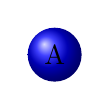
\begin{tikzpicture}[vertex/.style = {shape=circle, ball color=blue}]
    \node [vertex](A){A};
\end{tikzpicture}

% \begin{scope}[thick, draw=red]
%     \draw (1,1);
% \end{scope}
% \scoped[thick, draw=red]{\draw ...}
% {[thick, draw=red]
% \node (A) {A};
% }
\end{document}